\setcounter{equation}{0}
\chapter{Results}

\section{Influence of the viewing angle $\theta$}
As stated in the preceding chapter, we will also take into account the viewing angle of the galaxy to create the resulting spectra. So in order to proceed we will start stating the influence of this extra parameter in the \lya line. 

\begin{figure}[h!]
	\begin{center}
		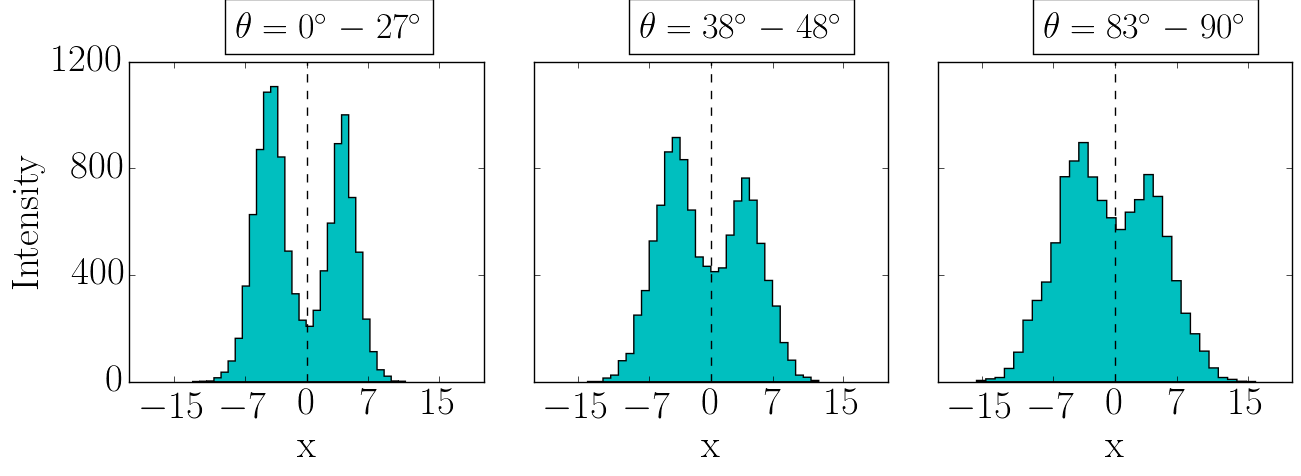
\includegraphics[width=1\textwidth]{./figures/chapter3/influence_viewing_angle2}
	\end{center}
	\caption{\textbf{\lya profile for different $\theta$:} With \tauh$=10^5$, \vrot$=50$ \kms and \vout$=20$ \kms.
		\label{fig:influence_viewing_angle}}
\end{figure}

It was noticed that for all of the different combinations that we ran, the effect of $\theta$ is always the same. For this, in order to exemplify we will use the particular case of \tauh$=10^5$, \vrot$=50$ \kms and \vout$=20$ \kms. As seen in Fig. \ref{fig:influence_viewing_angle} it is really clear that the intensity of the valley between the two peaks is increased along with $\theta$. This causes an intensity decrease in the rest of the frequencies, thus a broadening of the line. \\

Now, as the effect of the viewing angle is understood we can work from now on with a particular range of $\theta$ to decrease the number of cases. We ensure the reader it is an analogous behavior for all of them. In particular we will choose the range in which we see the galaxy's angular momentum vector going perpendicular to our relative position vector. In numbers this means: $\theta \in [83^\circ,96^\circ]$\\

\section{Runs}

Now, for each of the runs made we will explain how we narrowed our parameter space to obtain our final results. In all of the plots \vrot increases in the row from left to right and \vout increases in the column from top to bottom.\\ 

\newpage

\subsection{1st run}
In the 1st run we were focused on understanding what each parameter did to the line, more than its physical possibility to be present. For this we chose the values in the second column of Tab. \ref{tab:runs}. The obtained results are in Fig. \ref{fig:1_tau10E5_phi83-90} \ref{fig:1_tau10E6_phi83-90} and \ref{fig:1_tau10E7_phi83-90}.\\

\begin{figure}[h!]
	\begin{center}
		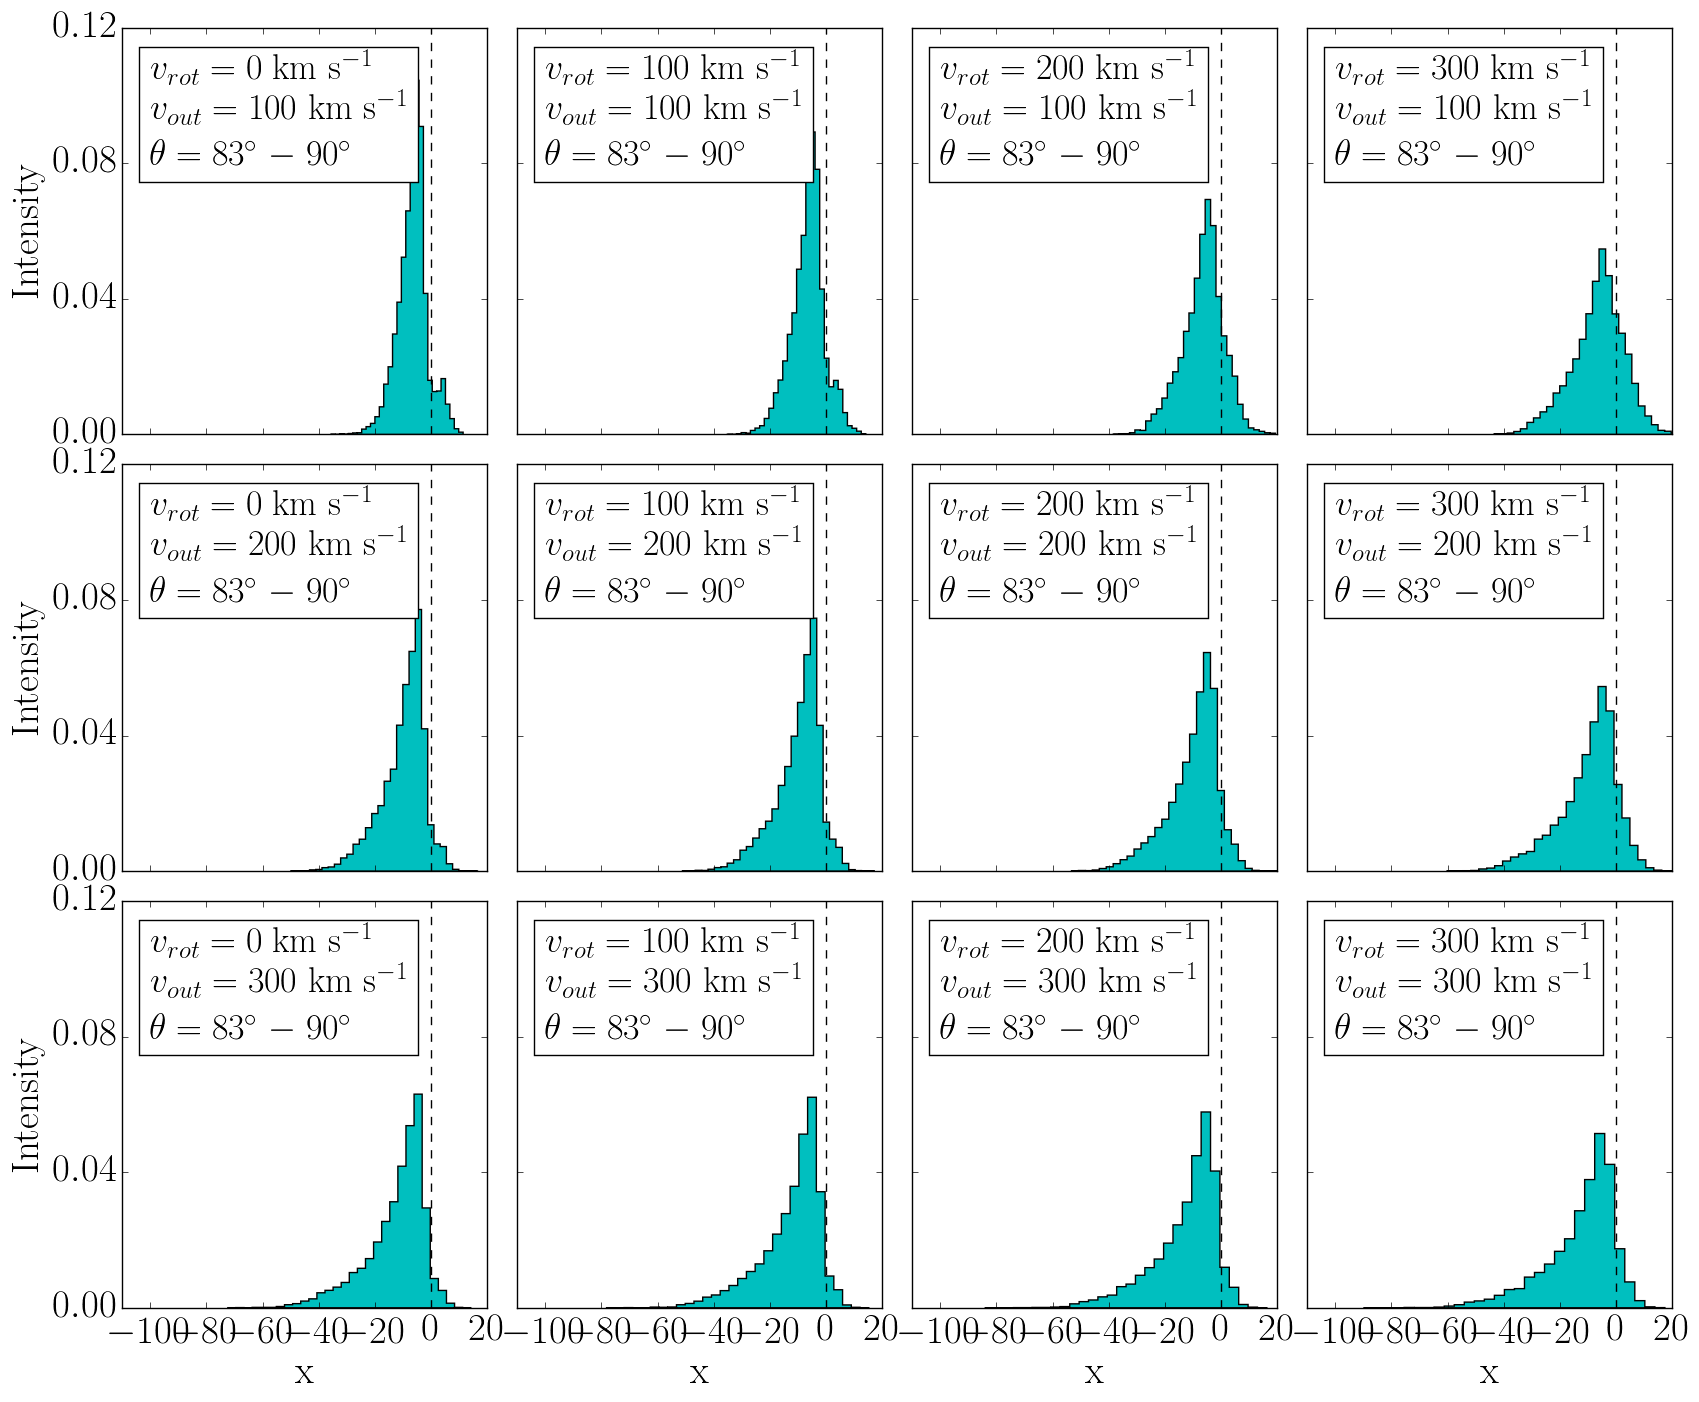
\includegraphics[width=1\textwidth]{./figures/chapter3/1_tau10E5_phi83-90}
	\end{center}
	\caption{\textbf{\lya profile for \tauh$=10^5$:} With \vrot ranging $0,100,200,300$ \kms and \vout ranging $100,200,300$ \kms.
		\label{fig:1_tau10E5_phi83-90}}
\end{figure}

\newpage

\begin{figure}[h!]
	\begin{center}
		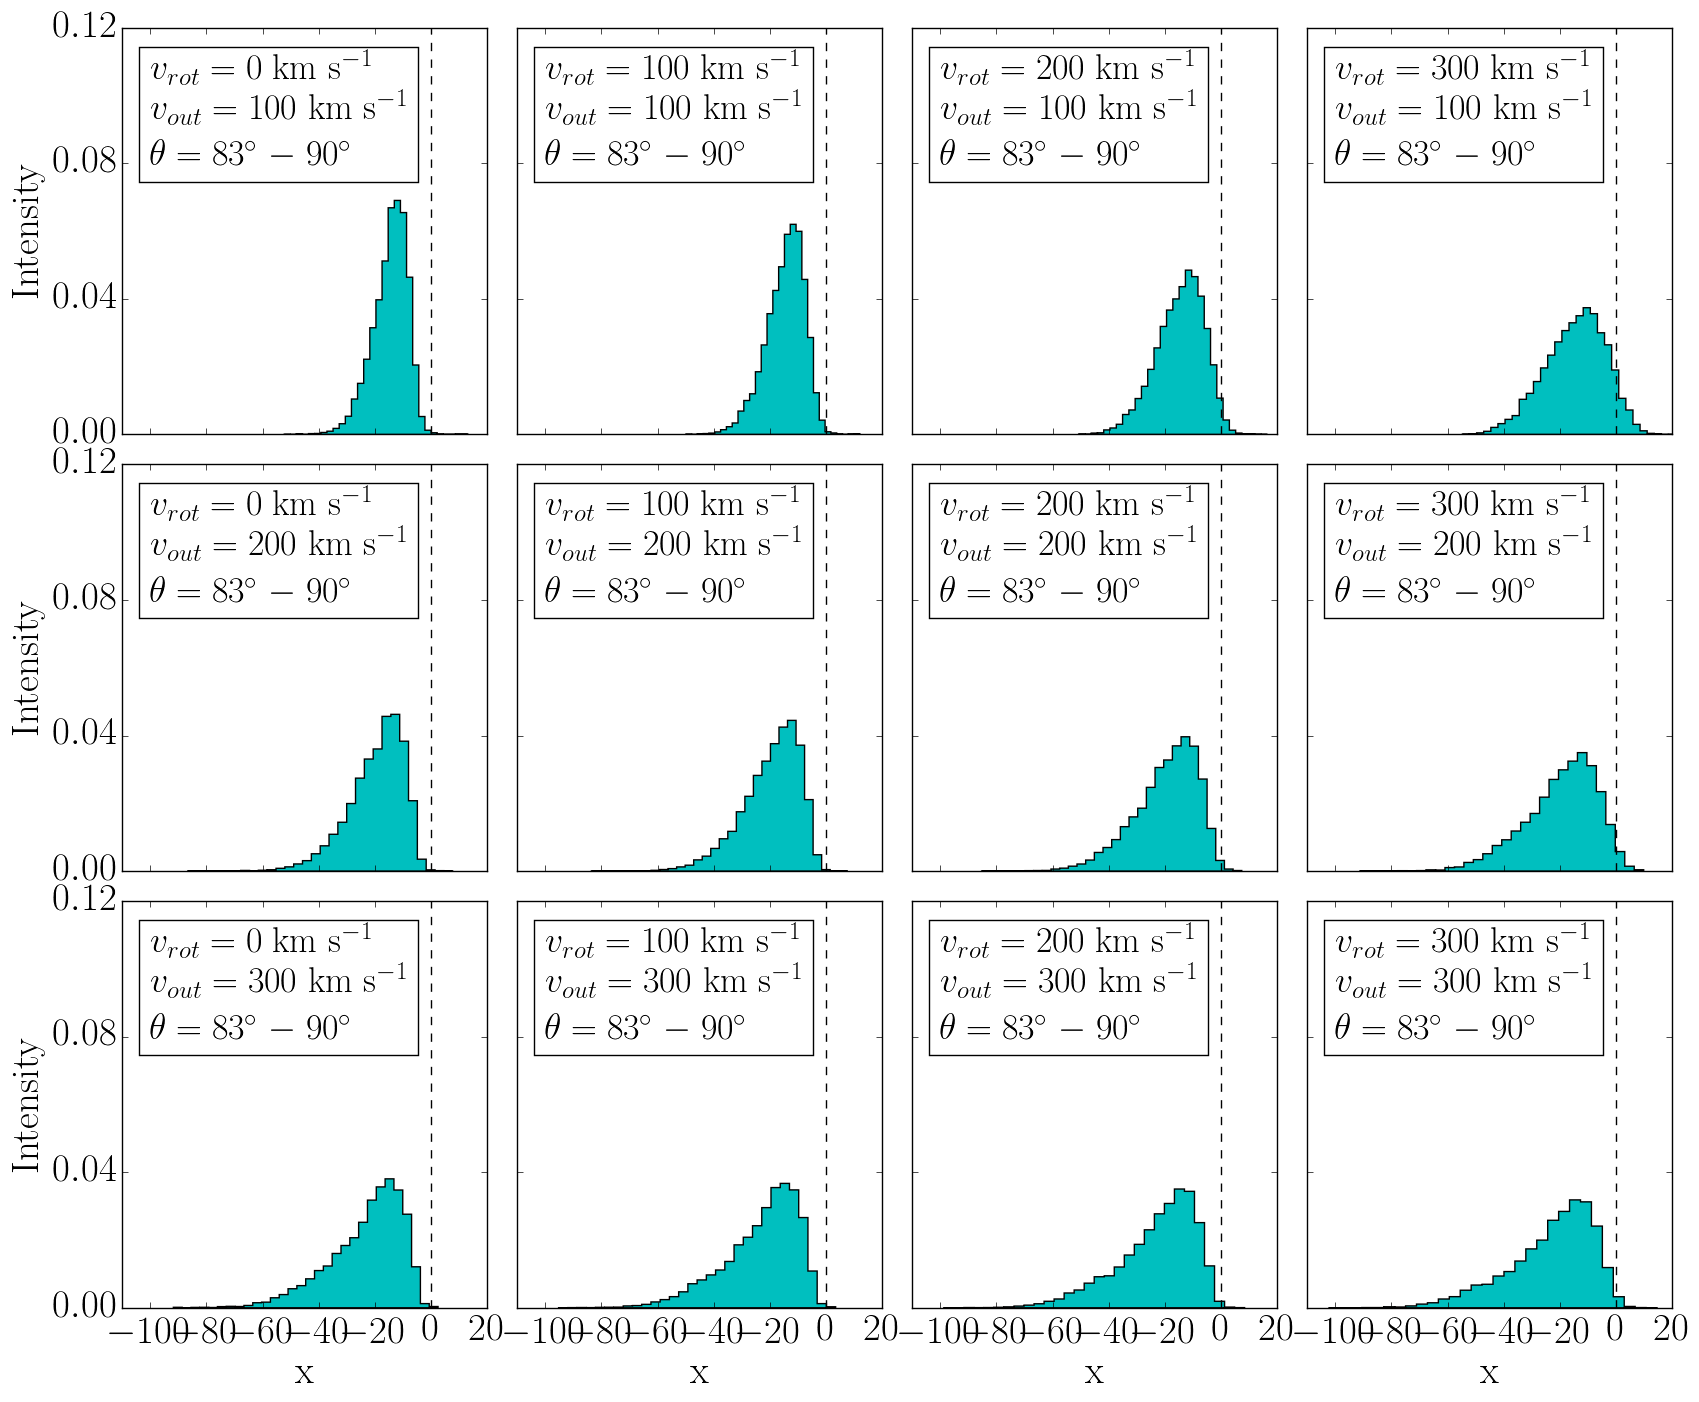
\includegraphics[width=1\textwidth]{./figures/chapter3/1_tau10E6_phi83-90}
	\end{center}
	\caption{\textbf{\lya profile for \tauh$=10^6$:} With \vrot ranging $0,100,200,300$ \kms and \vout ranging $100,200,300$ \kms.
		\label{fig:1_tau10E6_phi83-90}}
\end{figure}

\newpage

\begin{figure}[h!]
	\begin{center}
		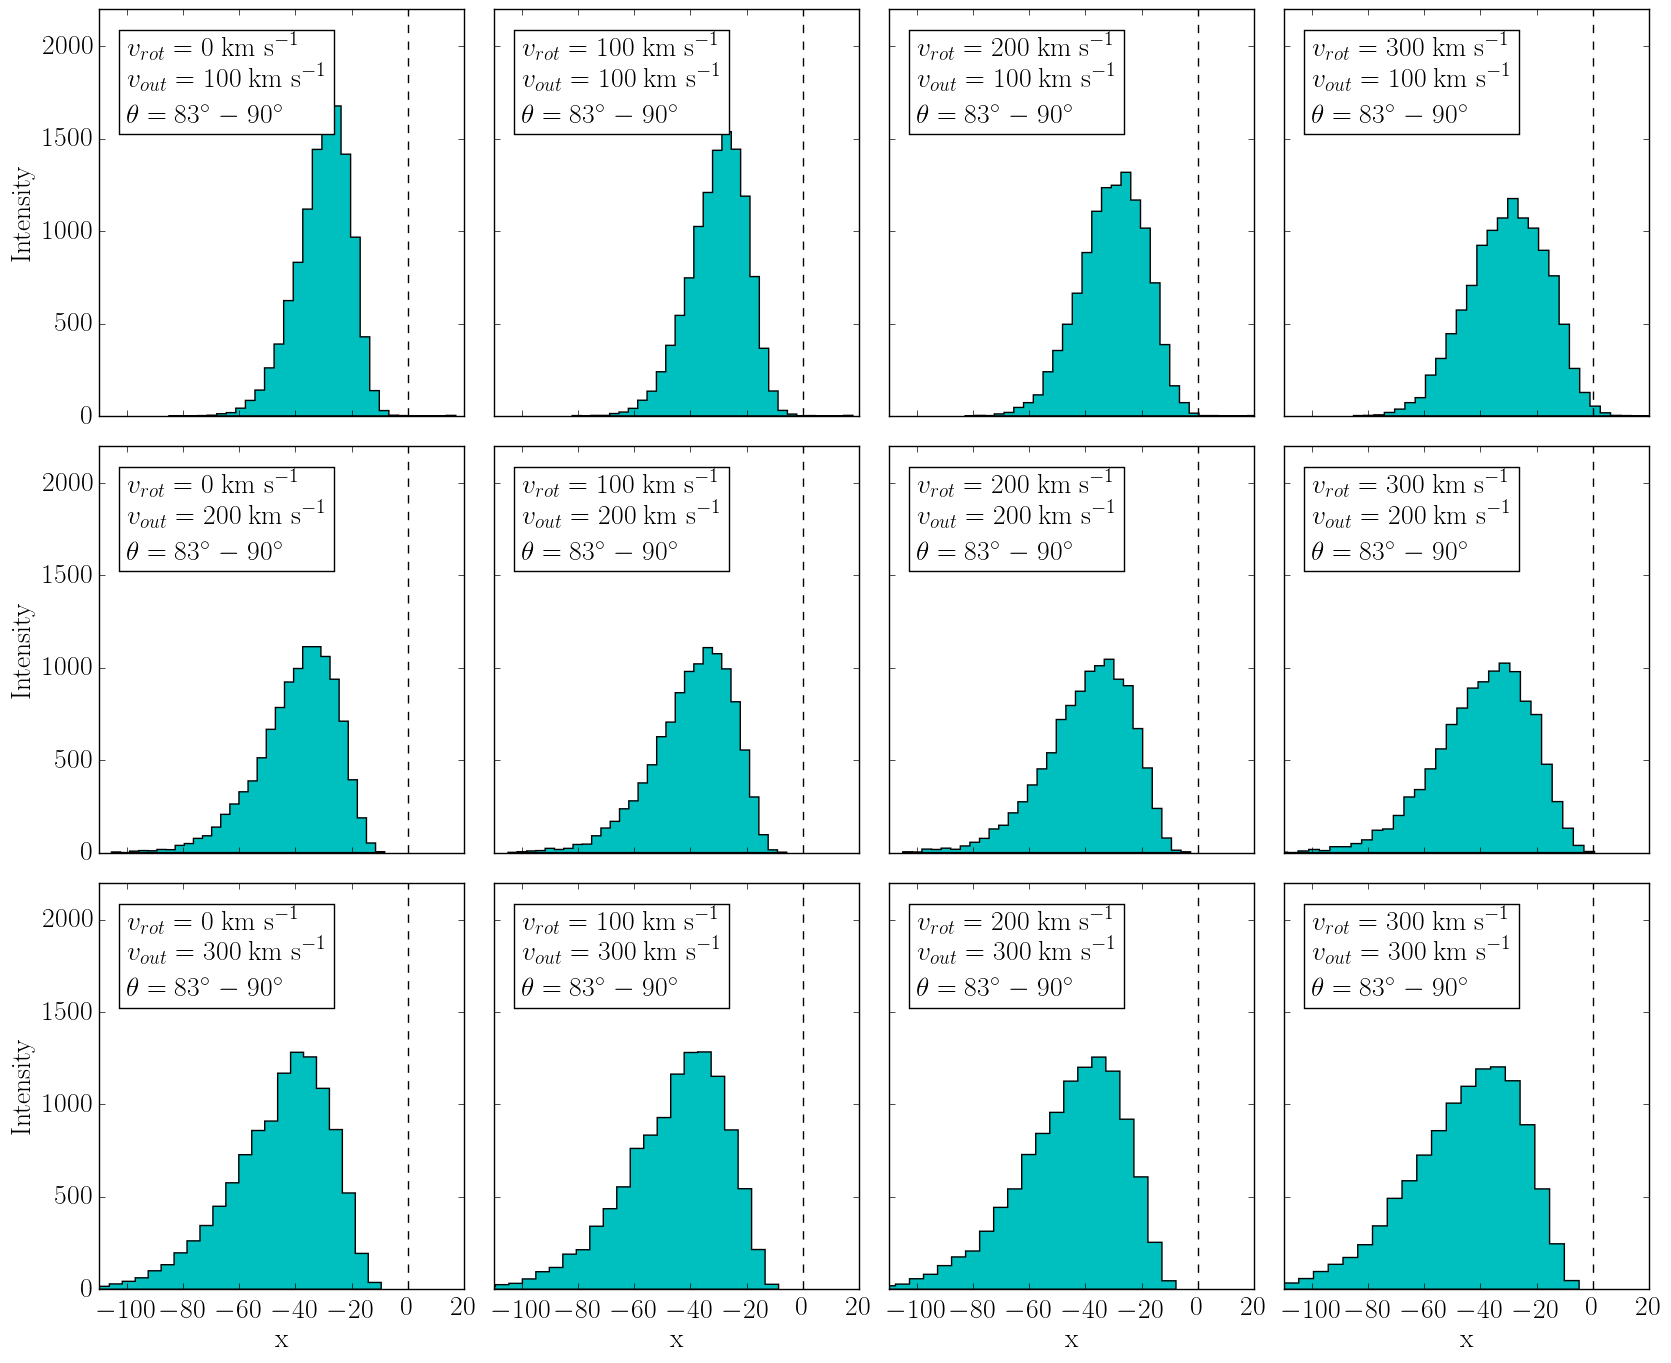
\includegraphics[width=1\textwidth]{./figures/chapter3/1_tau10E7_phi83-90}
	\end{center}
	\caption{\textbf{\lya profile for \tauh$=10^7$:} With \vrot ranging $0,100,200,300$ \kms and \vout ranging $100,200,300$ \kms.
		\label{fig:1_tau10E7_phi83-90}}
\end{figure}

In these three sets of figures (Fig. \ref{fig:1_tau10E5_phi83-90} \ref{fig:1_tau10E6_phi83-90} \ref{fig:1_tau10E7_phi83-90}) it is noted that most of the lines are a single peaks. However the effect of rotation should create two. Only in few squares the 2 peaks are visible but they are almost insignificant in comparison and there has to be low \vrot and \vout to obtain them. This means that the outflows effect so much larger than the other one, and in order to compare the influence of both is necessary to lower \vout. That is the purpose of the 2nd run.\\

\newpage

\subsection{2nd run}

In this run, the velocities were narrowed and much more physical parameters were selected. This last constrain means that the velocities are now consistent with the LAE's mass and typical properties. However the \vout is still relatively big compared to the \vrot. \\

\begin{figure}[h!]
	\begin{center}
		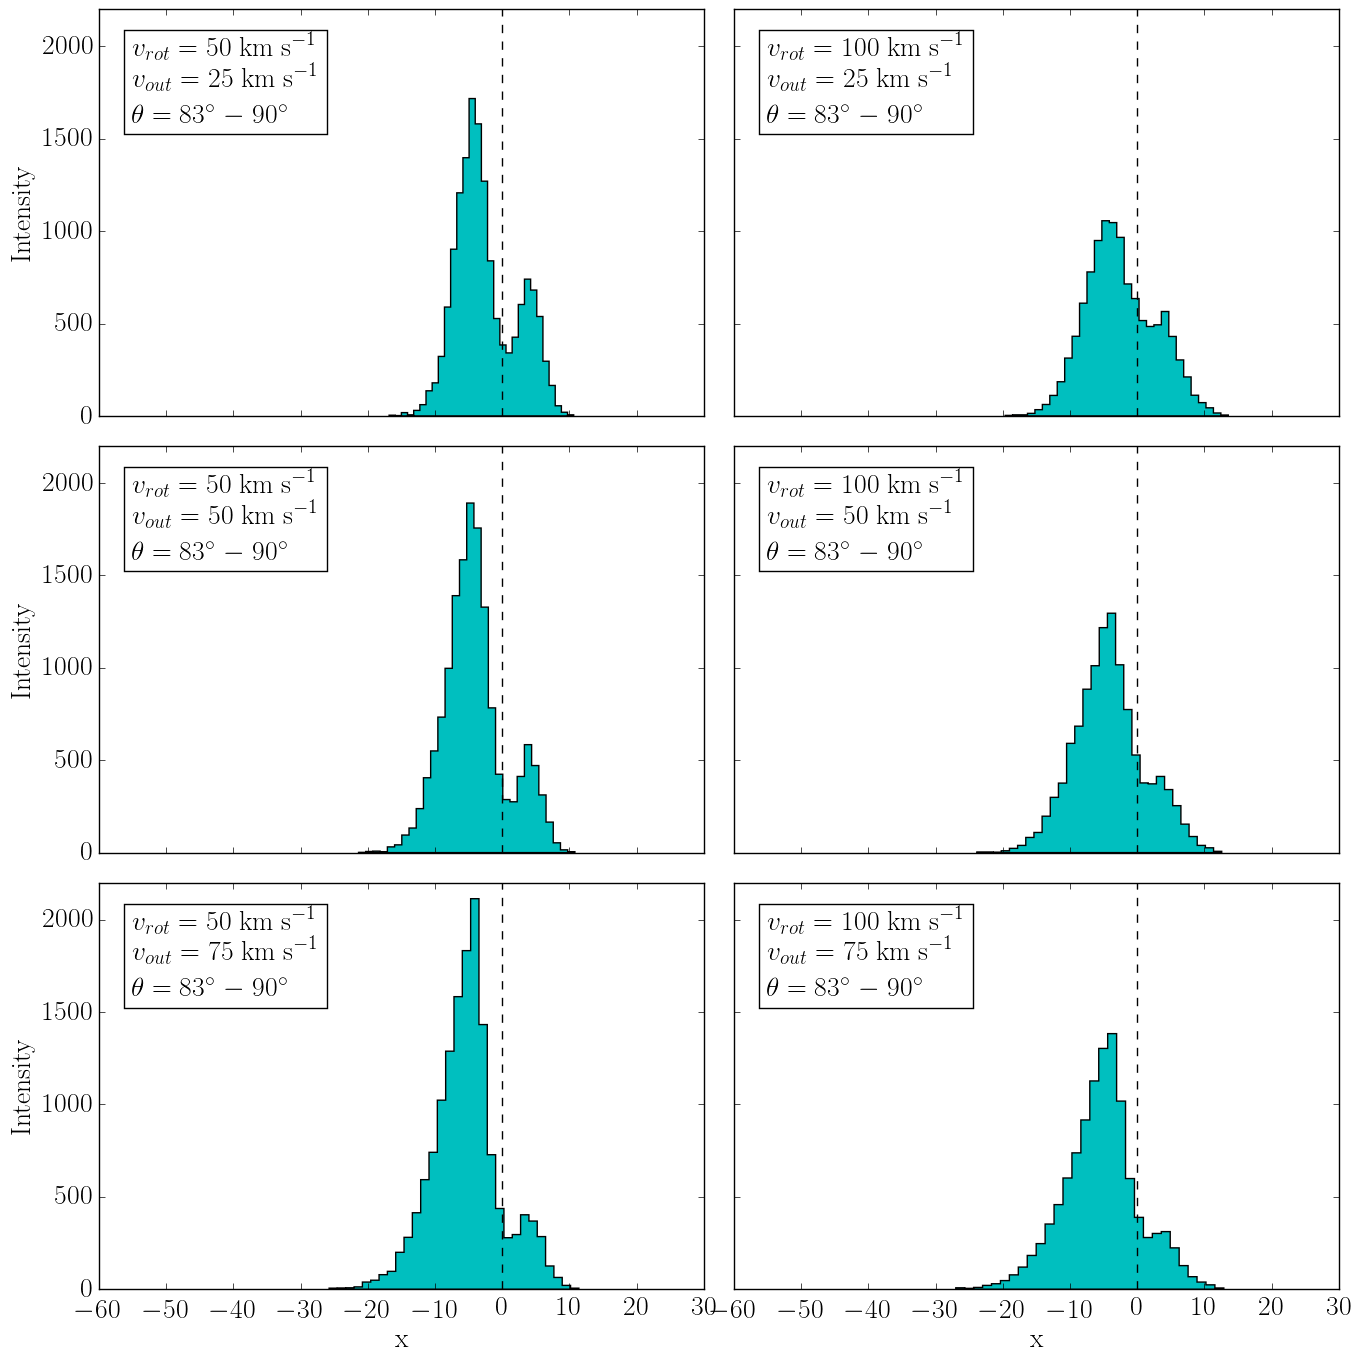
\includegraphics[width=1\textwidth]{./figures/chapter3/2_tau10E5_phi83-90}
	\end{center}
	\caption{\textbf{\lya profile for \tauh$=10^5$:} With \vrot ranging $50,100$ \kms and \vout ranging $25,50,75$ \kms.
		\label{fig:2_tau10E5_phi83-90}}
\end{figure}

\newpage

\begin{figure}[h!]
	\begin{center}
		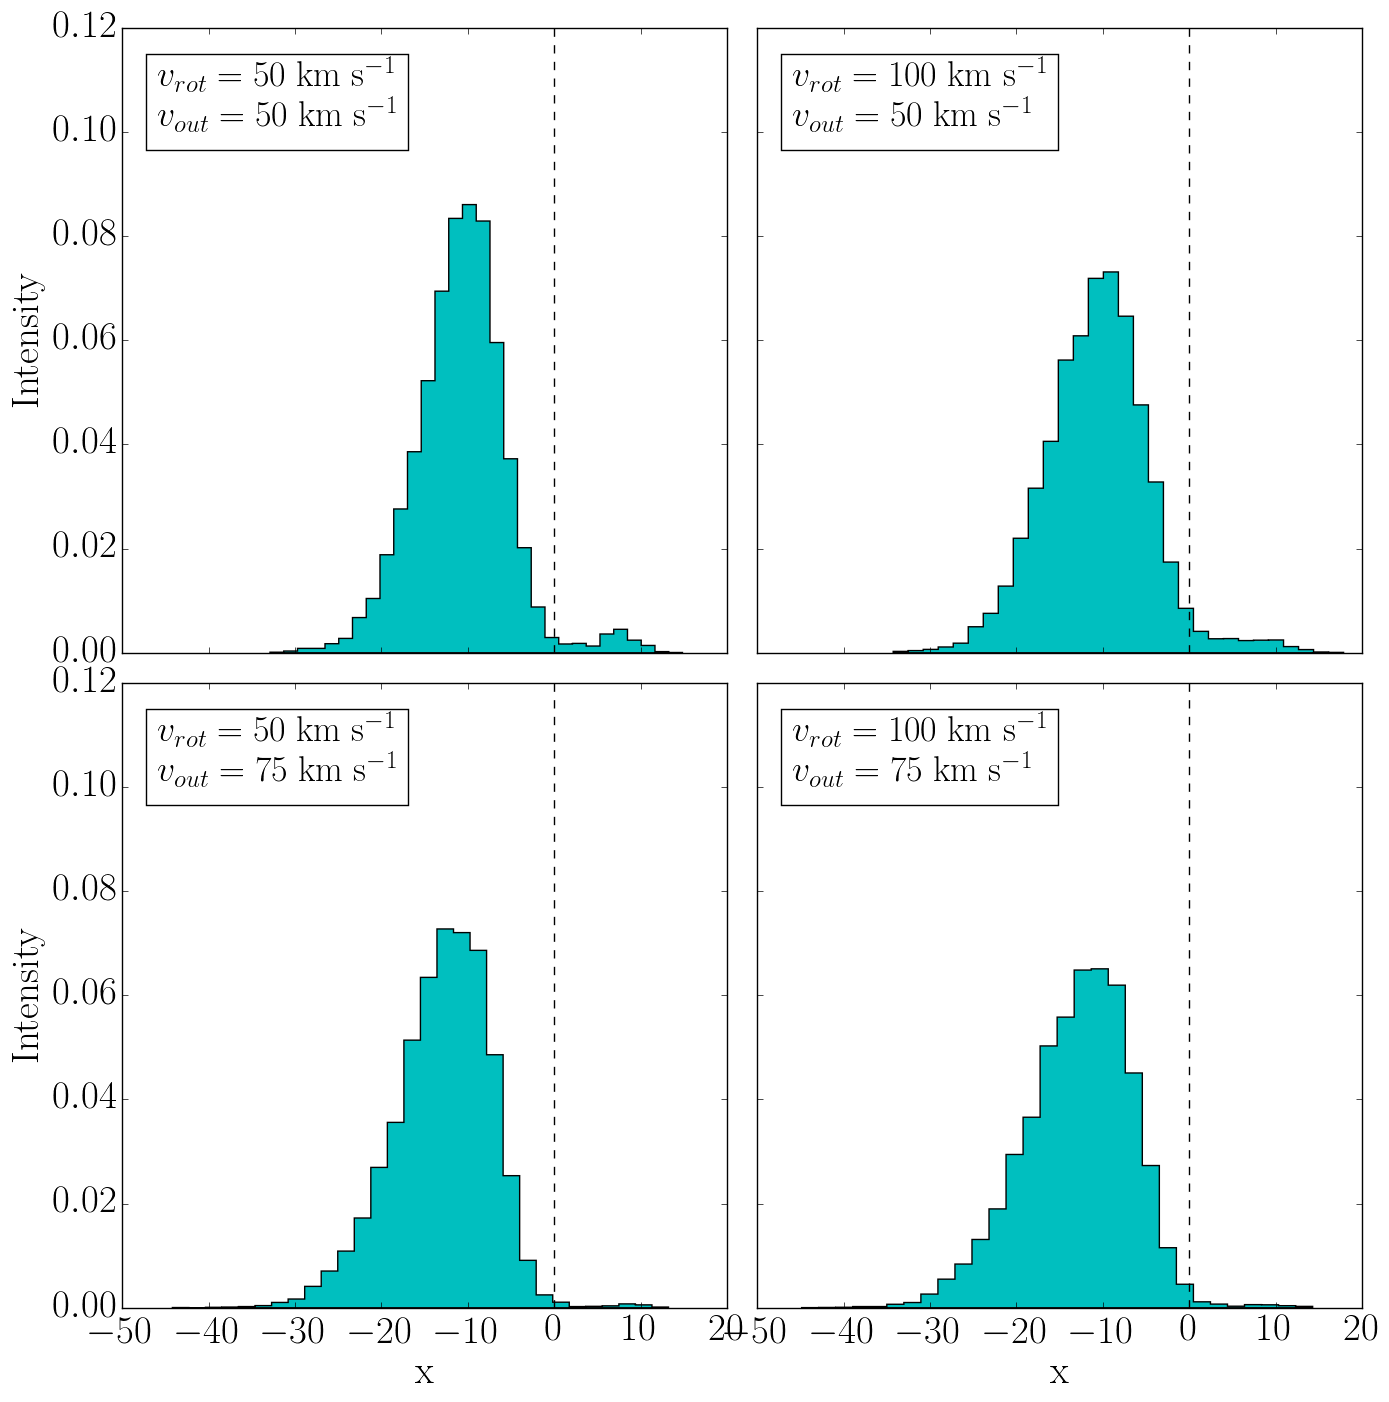
\includegraphics[width=1\textwidth]{./figures/chapter3/2_tau10E6_phi83-90}
	\end{center}
	\caption{\textbf{\lya profile for \tauh$=10^5$:} With \vrot ranging $50,100$ \kms and \vout ranging $25,50,75$ \kms.
		\label{fig:2_tau10E6_phi83-90}}
\end{figure}

\newpage

\begin{figure}[h!]
	\begin{center}
		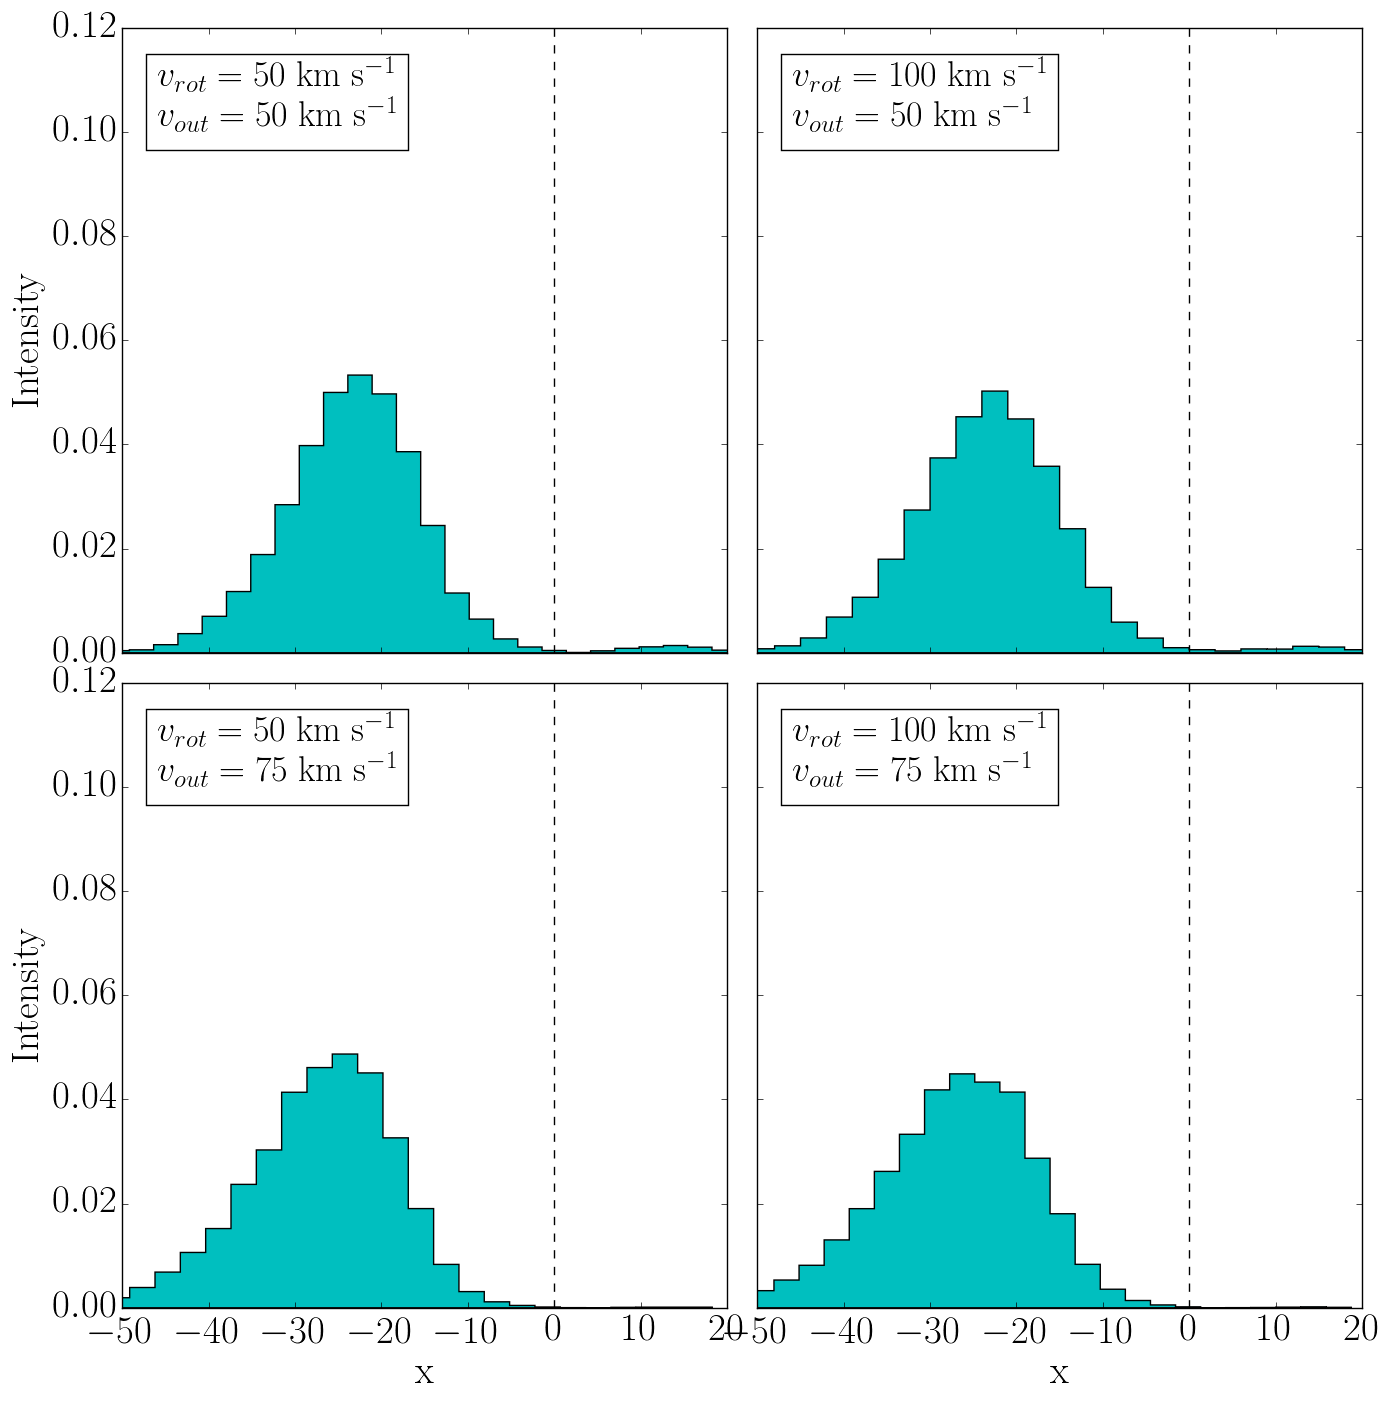
\includegraphics[width=1\textwidth]{./figures/chapter3/2_tau10E7_phi83-90}
	\end{center}
	\caption{\textbf{\lya profile for \tauh$=10^5$:} With \vrot ranging $50,100$ \kms and \vout ranging $25,50,75$ \kms.
		\label{fig:2_tau10E7_phi83-90}}
\end{figure}

In these three sets of figures (Fig. \ref{fig:2_tau10E5_phi83-90} \ref{fig:2_tau10E6_phi83-90} \ref{fig:2_tau10E7_phi83-90}) we can now see a clear second peak in more histograms. However when \vout/ \vrot $\geq 1$ the effect is negligible and can't still fully appreciate the rotation impact in the line. For this reason we had to run a 3rd set of parameters with \vout much smaller now. \\

\newpage

\subsection{3rd run}

In this run we took \vout below the lowest \vout of the 2nd run, but still the same \vrot as before. However as the magnitude of the velocity is now smaller, we did not run \tauh $=10^7$ because it wouldn't be consistent with it. \\

\begin{figure}[h!]
	\begin{center}
		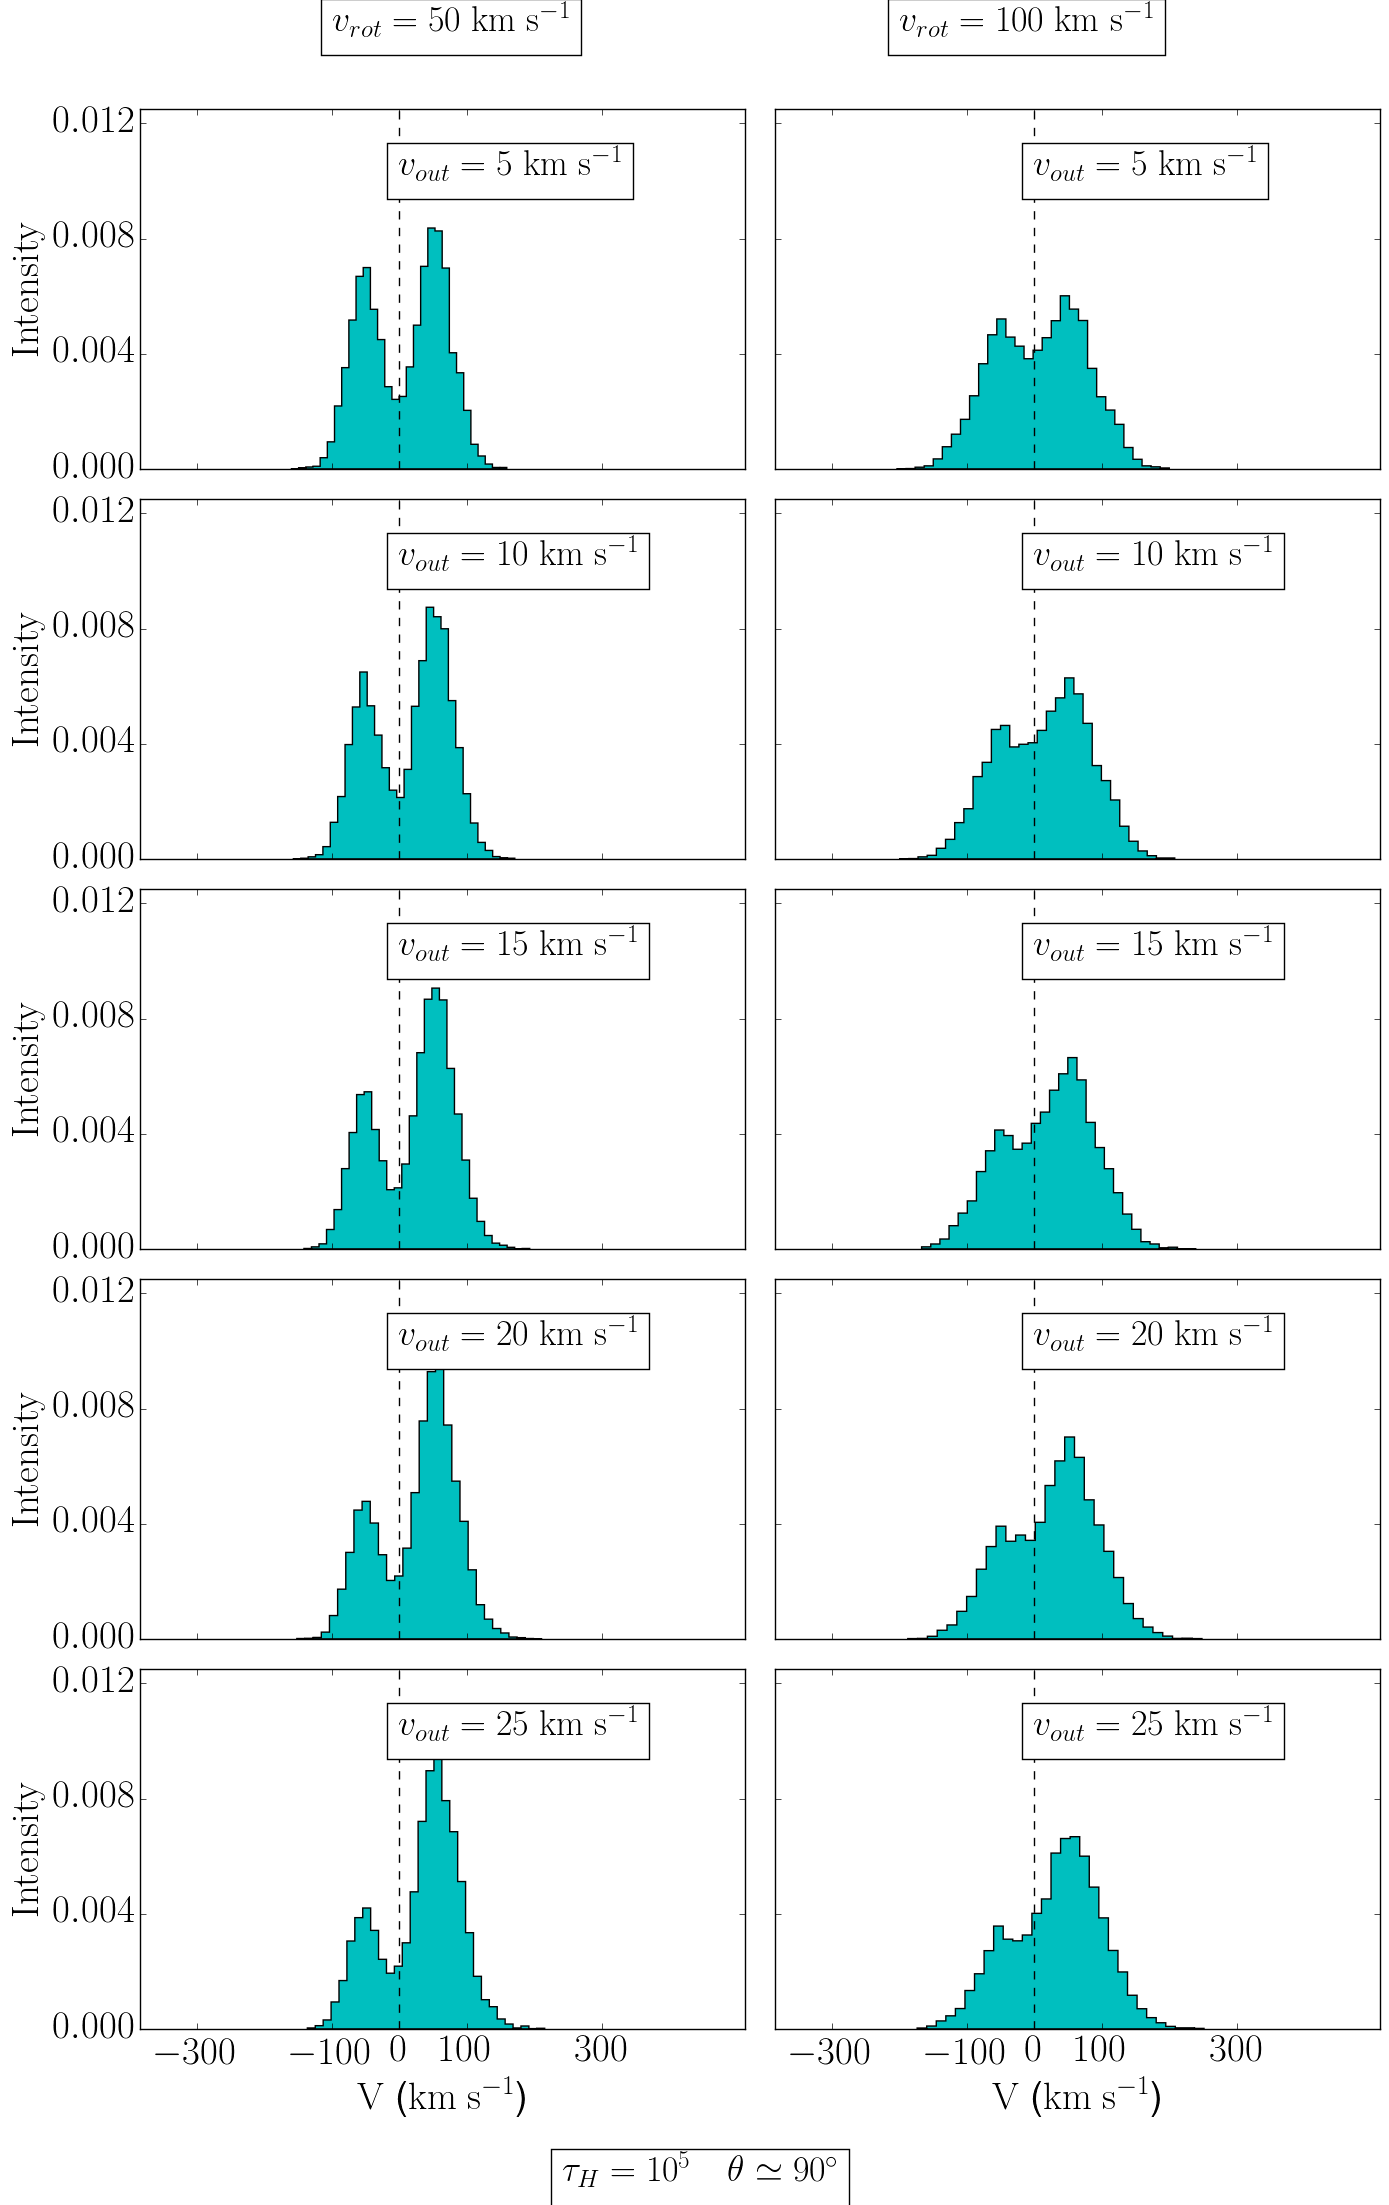
\includegraphics[width=0.9\textwidth]{./figures/chapter3/3_tau10E5_phi83-90}
	\end{center}
	\caption{\textbf{\lya profile for \tauh$=10^5$:} With \vrot ranging $50,100$ \kms and \vout ranging $5,10,15,20$ \kms.
		\label{fig:3_tau10E5_phi83-90}}
\end{figure}

\newpage

\begin{figure}[h!]
	\begin{center}
		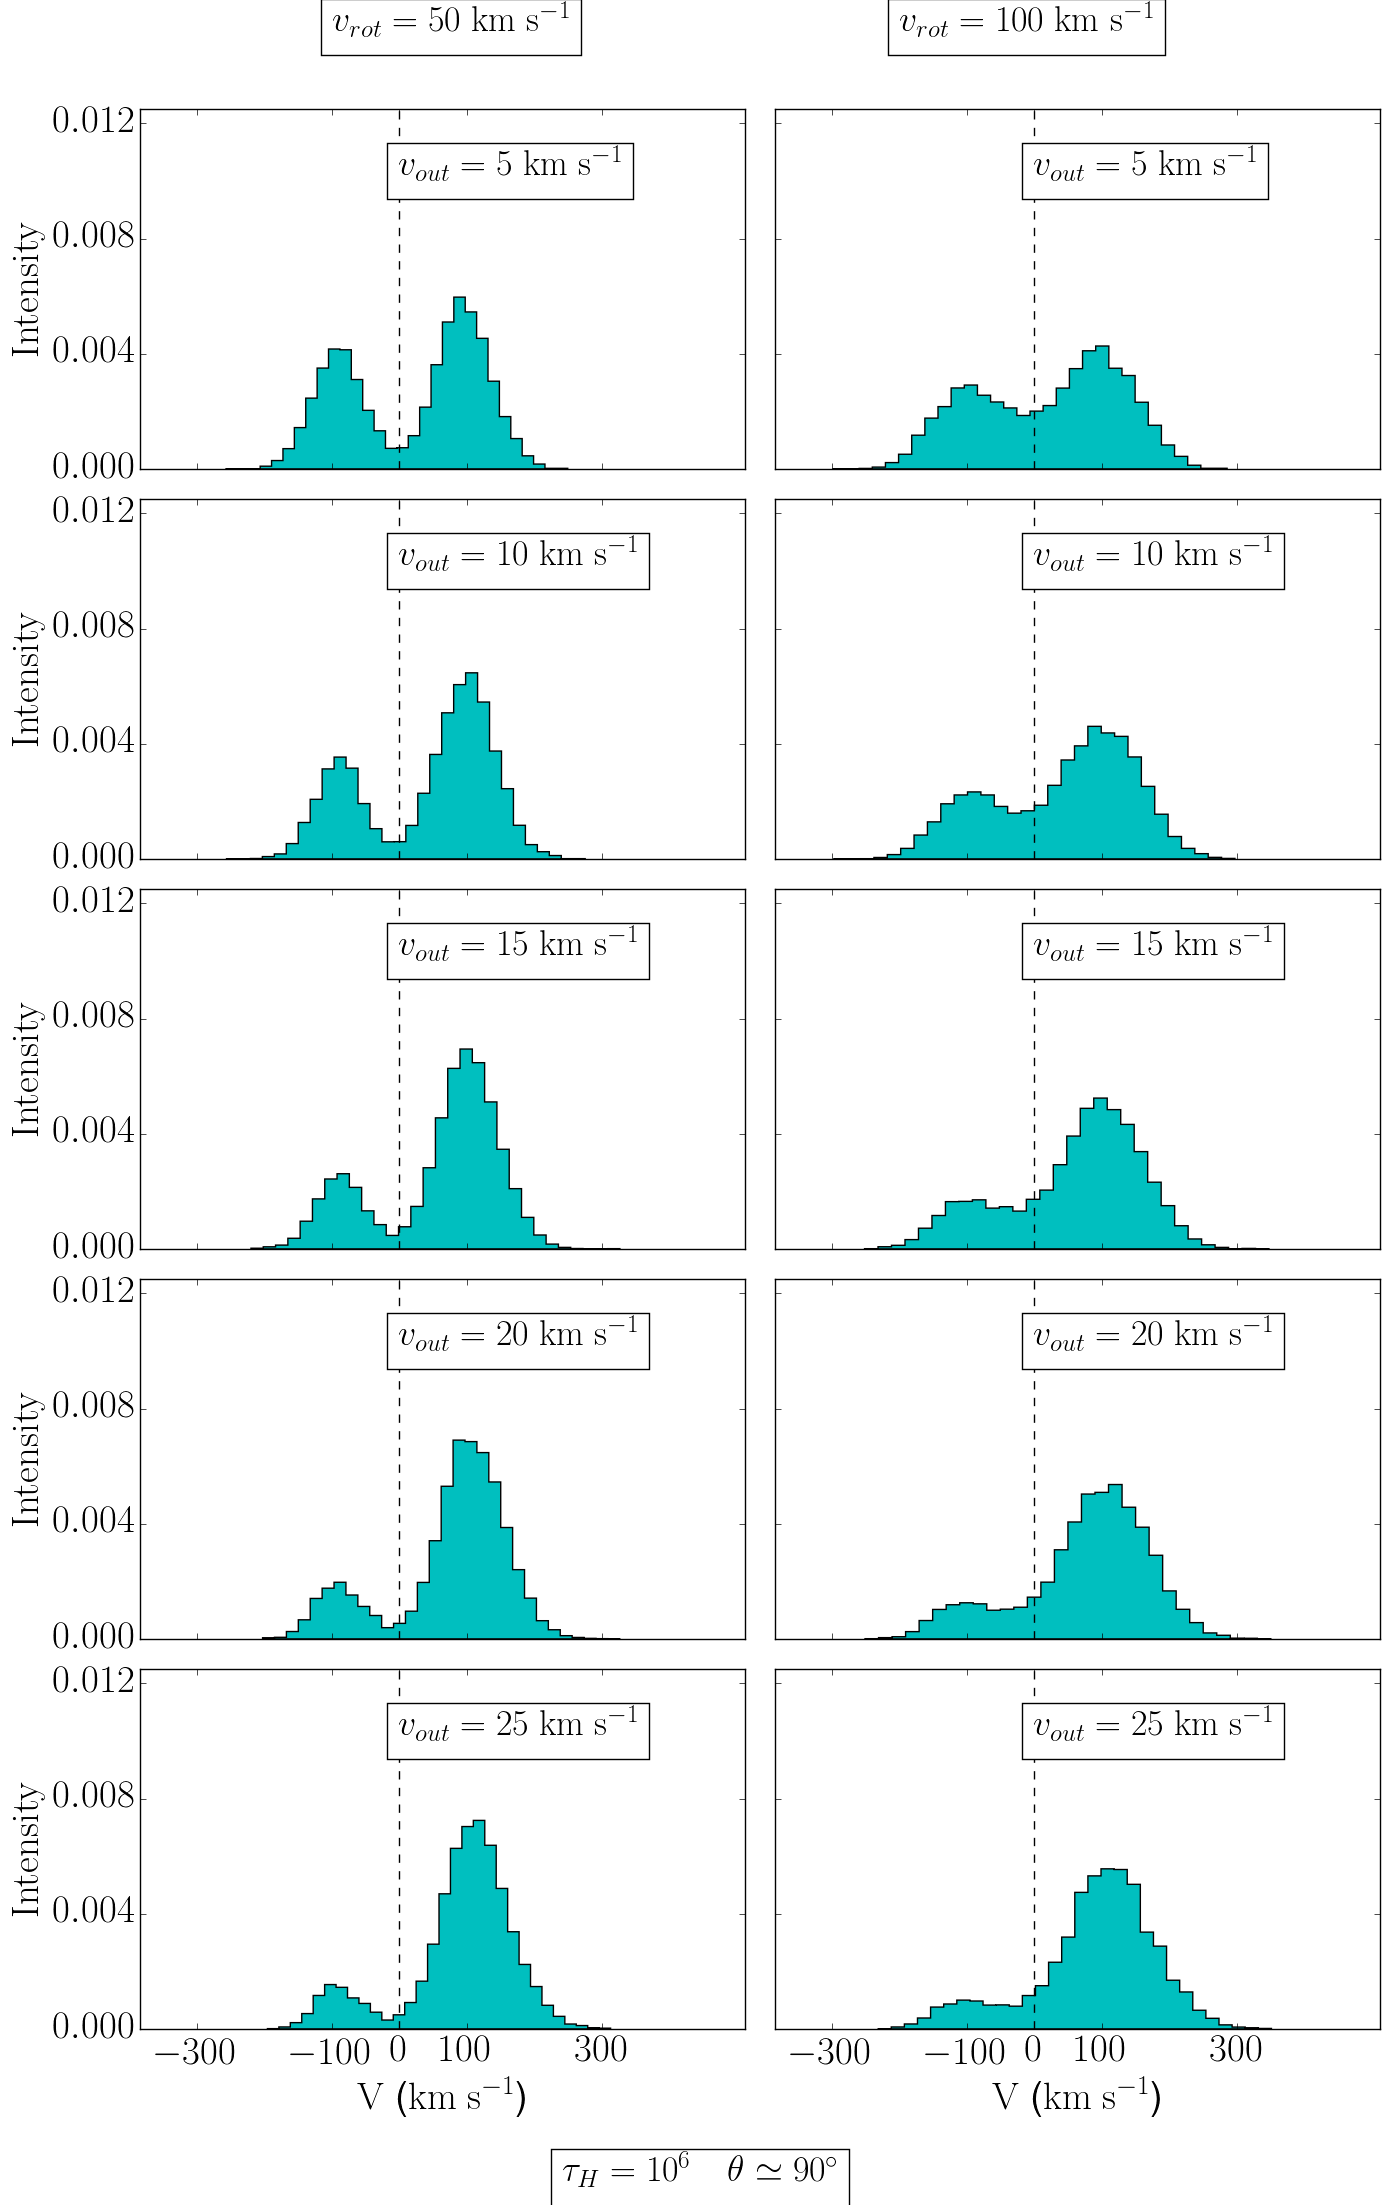
\includegraphics[width=0.9\textwidth]{./figures/chapter3/3_tau10E6_phi83-90}
	\end{center}
	\caption{\textbf{\lya profile for \tauh$=10^6$:} With \vrot ranging $50,100$ \kms and \vout ranging $5,10,15,20$ \kms.
		\label{fig:3_tau10E6_phi83-90}}
\end{figure}

These combinations of values make a lot more sense if we recall that \vout is caused mainly by starbursts, ejection of material out the galaxy. For this is not common that a galaxy expands faster than it rotates and from the figures (Fig. \ref{fig:3_tau10E5_phi83-90} \ref{fig:3_tau10E6_phi83-90}) we can confirm that only a little fraction of the \vrot radially is necessary to obtain 2 asymmetric peaks. \\

\section{Morphology of \lya line}
From now on, we will only show the results based on the 3rd run parameters combinations. In this section we will measure with 3 different quantities, the morphology of the \lya line in dependence of the velocities. First, we will use the standard deviation ($\mathrm{std}$), then the skewness ($\mathrm{skw}$) and finally a factor sigma of asymmetry ($\sigma_A$) defined by (MISSING REFERENCE).\\

\subsection{Standard Deviation}
In this part we will use the $\mathrm{std}$ to estimate the dispersion of the frequencies in the \lya line. Is important to recall that if the value is close to zero, then the frequencies tend to be very close to their expected value. If it increases, it means the frequencies are spreading to wider ranges. \\

\begin{figure}[h!]
	\begin{center}
		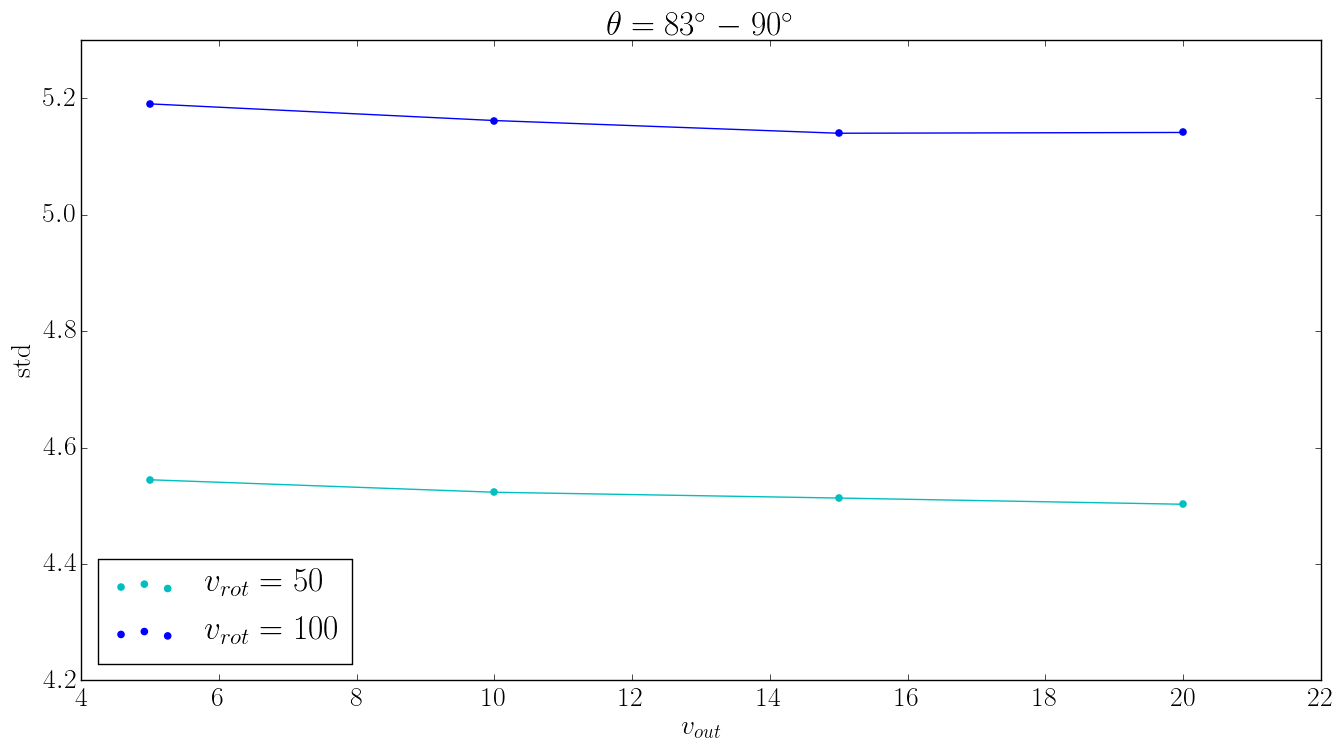
\includegraphics[width=1\textwidth]{./figures/chapter3/tau10E5_std_phi83-90}
	\end{center}
	\caption{\textbf{Skewness plot for \tauh$=10^5$.} 
		\label{fig:tau10E5_std_phi83-90}}
\end{figure}

\begin{figure}[h!]
	\begin{center}
		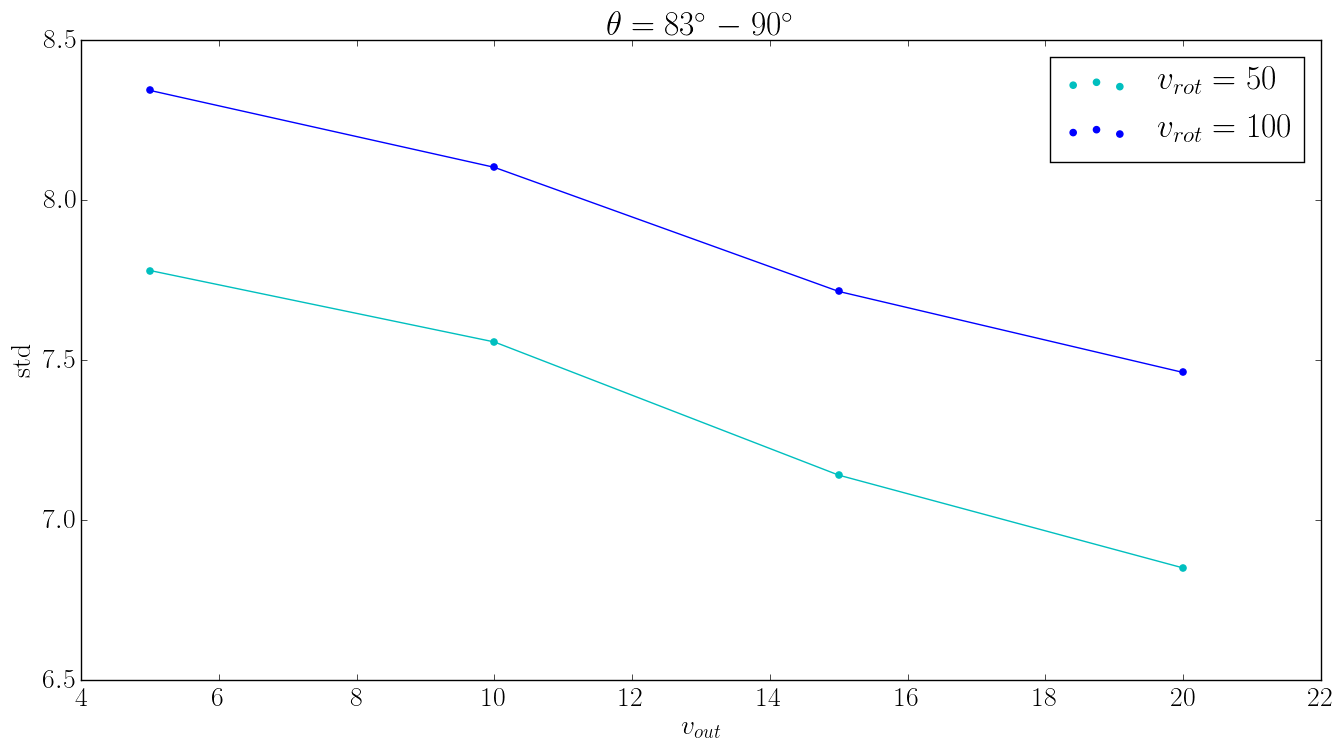
\includegraphics[width=1\textwidth]{./figures/chapter3/tau10E6_std_phi83-90}
	\end{center}
	\caption{\textbf{Skewness plot for \tauh$=10^6$.} 
		\label{fig:tau10E6_std_phi83-90}}
\end{figure}

As seen in figures (Fig. \ref{fig:tau10E5_std_phi83-90} \ref{fig:tau10E6_std_phi83-90}), the standard deviation is inversely proportional to the outflow velocity. And the higher the \tauh, the more inclined the curves. This implies that the greater \vout is, the less disperse the \lya frequency distribution. This clearly shows that the peaks start merging to one another it \vout is increasing.\\

\subsection{Skewness}
In this part we will use the $\mathrm{skw}$ to estimate the asymmetry of the \lya line. Is important to recall that if the value is greater than zero, there is more weight in the left tail of the line. And on the contrary, if it is less than zero, there is more weight in the right one.\\

\begin{figure}[h!]
	\begin{center}
		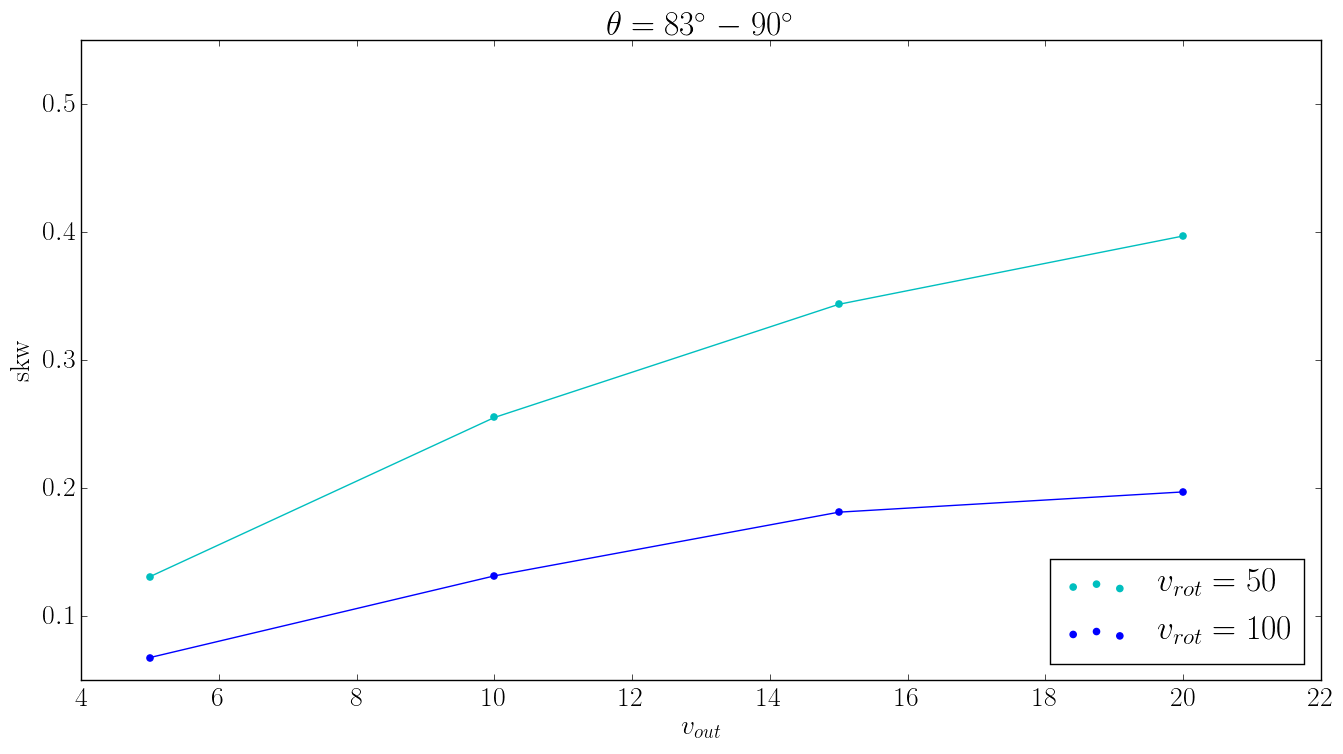
\includegraphics[width=1\textwidth]{./figures/chapter3/tau10E5_skw_phi83-90}
	\end{center}
	\caption{\textbf{Skewness plot for \tauh$=10^5$.} 
		\label{fig:tau10E5_skw_phi83-90}}
\end{figure}

\begin{figure}[h!]
	\begin{center}
		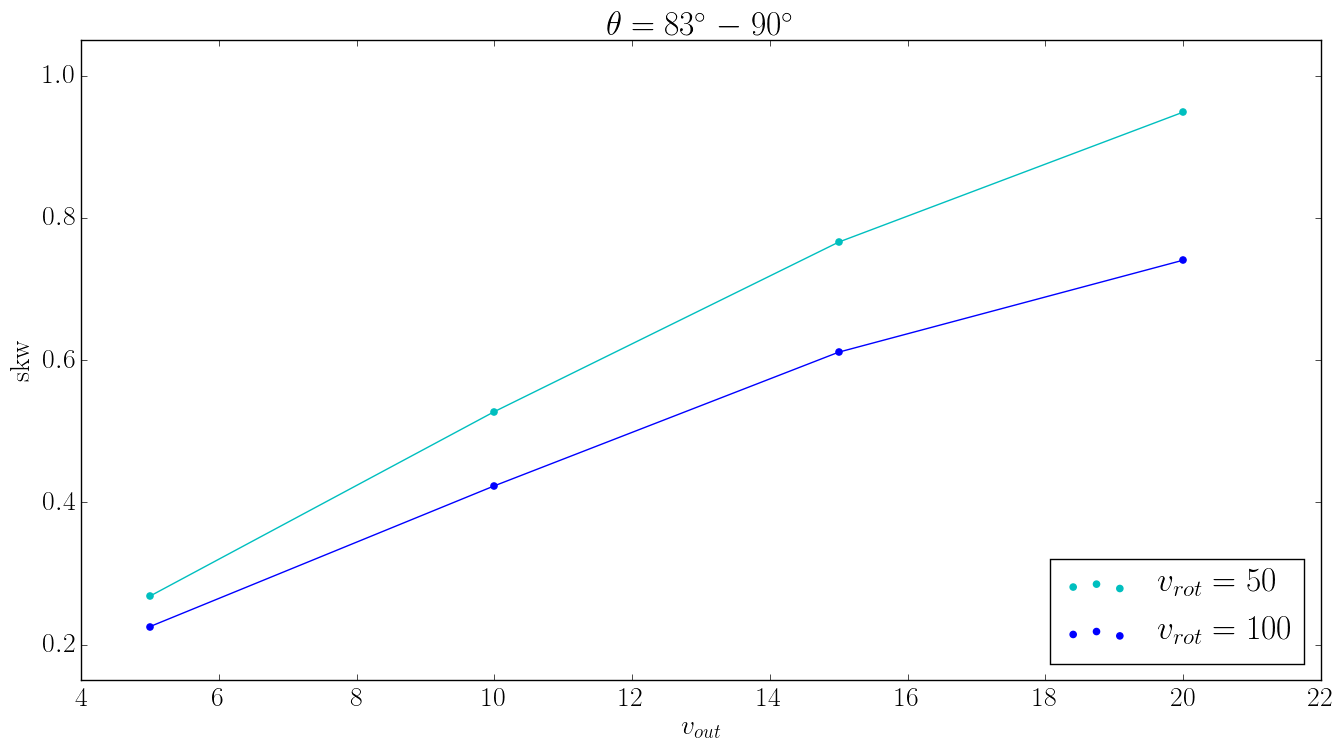
\includegraphics[width=1\textwidth]{./figures/chapter3/tau10E6_skw_phi83-90}
	\end{center}
	\caption{\textbf{Skewness plot for \tauh$=10^6$.} 
		\label{fig:tau10E6_skw_phi83-90}}
\end{figure}

As seen in figures (Fig. \ref{fig:tau10E5_skw_phi83-90} \ref{fig:tau10E6_skw_phi83-90}), the skewness is proportional to the outflow velocity. This implies that the greater \vout is, the more asymmetric is the \lya frequency distribution.\\

\subsection{Sigma of Asymmetry}
In this part we will use the $\sigma_A$ factor to estimate in another way the asymmetry of the \lya line. This was defined by (MISSING REFERENCE) as follows. The two peaks, the left one and the right one, are fitted with a Gaussian curve and their standard deviations $\sigma_{left}$ and $\sigma_{right}$ are obtained. Then the factor $\sigma_A$ is:

\begin{equation}
\sigma_A = \frac{\sigma_{right}}{\sigma_{left}}
\end{equation}

Is important to recall that if the value is greater than one, the left peak is thiner than the right peak. And if it is less than one, there left peak is wider than the right peak.\\

(MISSING PLOT)

%https://github.com/mariacamilaremolinagutierrez/RotationOutflowLymanAlpha/blob/master/Simulation/PeaksAsymmetry.ipynb

\section{Influences of the free parameters}

\subsection{Influence of the Galaxy Rotation Velocity: \vrot}
The influence of \vrot is slightly clear because of the giant impact \vout has. However it is noticeable that the \lya line broadens and lowers intensity when the rotation velocity increases. This result is consistent with Garavito et al. \cite{Garavito14}. \\

\subsection{Influence of the Galaxy Outflow Velocity: \vout}
The influence of \vout is very clear since the first run. When this outflows velocity increases, the right peak of the spectrum goes down in intensity until it merges with the left peak. \\

\subsection{Influence of the Galaxy Optical Depth: \tauh}
The influence of \tauh in the \lya line can be seen clearly in figures (Fig. \ref{fig:1_tau10E5_phi83-90} \ref{fig:1_tau10E6_phi83-90} \ref{fig:1_tau10E7_phi83-90}). What the optical depth causes is that the more \tauh there is, the more redshifted is the line respect to the zero value. \\